\chapter{Outer 动力学与有限 Inner 误差}
\label{chap:outer-dynamics}

第三章给出固定 prefix 下 KL 数值与梯度估计的条件误差。本章分析 inner 优化如何把这种误差传到 outer 同步后的策略，依次讨论精确 Gibbs 更新、PMD-Mean 更新、有限 inner、soft sync 和访问测度变化。沿用前两章的 $\pi_k$、$\pi_{k,n}$ 与 $\pi_T$；它们分别是冻结 anchor、inner student 和 teacher。

\section{Hard sync 的精确几何与稳定区间}
\label{sec:hard-sync-geometry}

本节固定一个 prefix，省略条件变量。沿用 $\pi_k$ 表示第 $k$ 轮冻结 anchor，$\pi_T$ 表示固定 teacher。词表 $\mathcal V$ 有限，$\pi_0(v)>0$、$\pi_T(v)>0$ 对所有 token 成立。假设 inner 优化确实得到 Gibbs target，随后将这个 target 完整复制为下一轮 anchor。这个假设同时排除了有限 inner 误差、模型表达能力不足和参数同步与分布同步之间的差异。

\begin{definition}[精确 Gibbs hard sync]
对任意 $\eta>0$ 和严格正分布 $\pi$，定义
\[
 T_\eta(\pi)(v)
 =\frac{\pi(v)^{1-\eta}\pi_T(v)^\eta}{Z_\eta(\pi)},
 \qquad
 Z_\eta(\pi)=\sum_{w\in\mathcal V}\pi(w)^{1-\eta}\pi_T(w)^\eta.
\]
精确 hard sync 是 $\pi_{k+1}=T_{\eta_k}(\pi_k)$。$\eta_k$ 是 mirror 更新的步长；它与优化器学习率及每轮 inner steps 是不同量。
\end{definition}

严格正性使负指数也有定义。因此本节先分析所有 $\eta>0$ 的数学更新，再区分通常采用的 $0<\eta\leq1$ 区间。若初始分布有零概率，$0<\eta<1$ 的更新会一直保留这些零概率，不能恢复 teacher 的完整支持集；$\eta>1$ 的负幂则在这些 token 上失去定义。有限 logits 的 softmax 满足正性，而显式截断后的采样分布不能直接代入本节结论。

\subsection{归一化常数消去后的精确收缩}

\begin{definition}[Log-ratio 跨度与 Hilbert 距离]
对 token 函数 $f$，定义
\[
 \operatorname{osc}_v f_v=\max_v f_v-\min_v f_v.
\]
对两个严格正概率分布，定义
\[
 d_H(\pi,\widetilde\pi)
 =\operatorname{osc}_v\log\frac{\pi(v)}{\widetilde\pi(v)},
 \qquad b_k=d_H(\pi_k,\pi_T).
\]
$d_H$ 是正概率单纯形上的 Hilbert 距离。它忽略 log-density 中与 token 无关的加性常数，恰好对应概率归一化所消除的自由度。
\end{definition}

这个定义确实给出距离。非负性来自最大值减最小值；对称性来自 $\operatorname{osc}(-f)=\operatorname{osc}(f)$；三角不等式来自 $\operatorname{osc}(f+g)\leq\operatorname{osc}(f)+\operatorname{osc}(g)$。若 $d_H(\pi,\widetilde\pi)=0$，则两个分布的概率比是常数，归一化迫使这个常数等于一。

\begin{theorem}[两条 hard-sync 轨迹的精确收缩]
\label{thm:hs-pairwise-contraction}
相同 teacher 和相同步长下，任意严格正分布满足
\begin{equation}\label{eq:hs-pairwise-contraction}
 d_H(T_\eta(\pi),T_\eta(\widetilde\pi))
 =|1-\eta|d_H(\pi,\widetilde\pi).
\end{equation}
特别地，$\pi_T$ 是不动点，而且
\[
 b_{k+1}=|1-\eta_k|b_k.
\]
\end{theorem}

\begin{proof}
先逐 token 相除，再取对数：
\[
 \log\frac{T_\eta(\pi)(v)}{T_\eta(\widetilde\pi)(v)}
 =(1-\eta)\log\frac{\pi(v)}{\widetilde\pi(v)}
 -\log Z_\eta(\pi)+\log Z_\eta(\widetilde\pi).
\]
最后两个项与 token 无关，在跨度中抵消。对任意实数 $c$，$\operatorname{osc}(cf)=|c|\operatorname{osc}(f)$，从而得到式~\eqref{eq:hs-pairwise-contraction}。将 $\widetilde\pi=\pi_T$ 代入，并使用 $T_\eta(\pi_T)=\pi_T$，得到第二个结论。
\end{proof}

\begin{theorem}[常步长与变步长的精确解]
\label{thm:hard-sync}
记
\[
 A_0=1,\qquad A_k=\prod_{j=0}^{k-1}(1-\eta_j),
 \qquad u_v=\log\frac{\pi_0(v)}{\pi_T(v)}.
\]
任意正步长序列的精确解为
\begin{equation}\label{eq:hard-closed}
 \pi_k(v)=\frac{\pi_T(v)e^{A_k u_v}}
 {\sum_w\pi_T(w)e^{A_k u_w}},
 \qquad b_k=|A_k|b_0.
\end{equation}
常步长时 $A_k=(1-\eta)^k$，也可以写成
\[
 \pi_k(v)=\frac{\pi_0(v)^{(1-\eta)^k}
 \pi_T(v)^{1-(1-\eta)^k}}
 {\sum_w\pi_0(w)^{(1-\eta)^k}
 \pi_T(w)^{1-(1-\eta)^k}}.
\]
\end{theorem}

\begin{proof}
$k=0$ 时 $\pi_T(v)e^{u_v}=\pi_0(v)$，配分函数等于一。假设第 $k$ 轮公式成立，其归一化常数记为 $C_k$。下一轮未归一化权重为
\begin{align*}
 \pi_k(v)^{1-\eta_k}\pi_T(v)^{\eta_k}
 &=C_k^{-(1-\eta_k)}\pi_T(v)
       e^{(1-\eta_k)A_k u_v}\\
 &=C_k^{-(1-\eta_k)}\pi_T(v)e^{A_{k+1}u_v}.
\end{align*}
第一项不依赖 token，归一化后消失。由归纳得到分布闭式。取相对 teacher 的 log-ratio 后，归一化常数同样在跨度中抵消，得到 $b_k=|A_k|b_0$。
\end{proof}

\begin{corollary}[常步长的完整稳定分类]
对非 teacher 初值，精确 hard sync 的行为如下。
\begin{enumerate}
 \item $0<\eta<1$ 时，$A_k>0$ 且趋于零，策略从同一侧趋向 teacher。
 \item $\eta=1$ 时，第一轮更新等于 teacher，此后保持不变。
 \item $1<\eta<2$ 时，$A_k$ 正负交替并趋于零，策略在 teacher 两侧交替收敛。
 \item $\eta=2$ 时，$A_k=(-1)^k$，形成精确二周期。
 \item $\eta>2$ 时，$|A_k|$ 发散，log-ratio 跨度发散，策略不能趋向 teacher。
\end{enumerate}
因此完整的全局渐近稳定区间是 $0<\eta<2$。teacher KL 的每步单调下降需要另外分析。
\end{corollary}

\begin{proof}
前四项直接由式~\eqref{eq:hard-closed} 得到。第五项中，偶数轮的 $A_k$ 趋于正无穷，奇数轮趋于负无穷。偶数轮的概率质量集中到 $u_v$ 最大的 token 集合，奇数轮集中到最小的 token 集合；各集合内部的极限概率与 $\pi_T$ 成比例。非 teacher 初值使 $u$ 非常数，所以两个集合互不相交。

有限正 teacher 下仍有
\[
 \KL(\pi_k\Vert\pi_T)\leq\log\frac1{\min_v\pi_T(v)}.
\]
因此这里发散的是 log-ratio 跨度和反向 KL，而正向 teacher KL 保持有界。反向 KL 发散，是因为上述集中使某些具有正 teacher 质量的 token 概率趋于零。
\end{proof}

\begin{proposition}[变步长的充要条件]
非 teacher 初值下，$\pi_k\to\pi_T$ 当且仅当 $A_k\to0$。若每个 $\eta_k\in(0,2)$，且没有任何一步等于一，则这个条件等价于
\[
 \sum_{k=0}^{\infty}\eta_k(2-\eta_k)=\infty.
\]
若某一步等于一，则此后 $A_k=0$，直接收敛。
\end{proposition}

\begin{proof}
$A_k\to0$ 时由有限词表闭式得到逐 token 收敛。反过来，概率趋向严格正 teacher 时 $b_k\to0$；因为 $b_0>0$，故 $|A_k|\to0$。对 $a_k=|1-\eta_k|\in(0,1)$，无限乘积 $\prod_k a_k$ 为零，当且仅当 $\sum_k(1-a_k)$ 发散。这个标准乘积判据可以由 $-\log a\geq1-a$，以及 $a$ 接近一时 $-\log a\leq2(1-a)$ 推出。最后使用
\[
 1-a_k\leq1-a_k^2\leq2(1-a_k),
 \qquad 1-a_k^2=\eta_k(2-\eta_k),
\]
得到等价条件。
\end{proof}

例如 $\eta_k=1/(k+2)$ 给出 $A_K=1/(K+1)\to0$。若改成 $\eta_k=1/(k+2)^2$，则
\[
 A_K=\prod_{n=2}^{K+1}\frac{(n-1)(n+1)}{n^2}
 =\frac{K+2}{2(K+1)}\longrightarrow\frac12.
\]
第二种步长虽然每轮都执行正确方向的 hard sync，但总更新量有限，最终仍保留初始 log-ratio 的一半。

\subsection{配分函数与两个方向的 KL 路径}

沿用上节 $u_v$，定义一条由初始策略和 teacher 唯一确定的路径：
\[
 \psi(a)=\log\sum_v\pi_T(v)e^{a u_v},\qquad
 \pi^{[a]}(v)=\pi_T(v)e^{a u_v-\psi(a)}.
\]
这里 $a$ 是路径坐标，实际第 $k$ 轮取 $a=A_k$；它不代表新的策略变量。归一化给出 $\psi(0)=\psi(1)=0$，以及 $\pi^{[0]}=\pi_T$、$\pi^{[1]}=\pi_0$。

\begin{theorem}[KL 路径的精确积分]
\label{thm:hs-kl-path}
配分函数满足
\[
 \psi'(a)=\E_{\pi^{[a]}}u,
 \qquad\psi''(a)=\Var_{\pi^{[a]}}(u).
\]
沿路径的正向与反向 KL 分别为
\begin{align}
 \KL(\pi^{[a]}\Vert\pi_T)
 &=a\psi'(a)-\psi(a)
 =\int_0^a z\psi''(z)\,\mathrm dz,
 \label{eq:hs-forward-kl-path}\\
 \KL(\pi_T\Vert\pi^{[a]})
 &=\psi(a)-a\psi'(0)
 =\int_0^a(a-z)\psi''(z)\,\mathrm dz.
 \label{eq:hs-reverse-kl-path}
\end{align}
任意路径两点之间还有
\[
 \KL(\pi^{[a]}\Vert\pi^{[c]})
 =(a-c)\psi'(a)-\psi(a)+\psi(c).
\]
\end{theorem}

\begin{proof}
有限词表允许逐项微分。令 $C(a)=\sum_v\pi_T(v)e^{au_v}$，则
\[
 \psi'(a)=\frac{C'(a)}{C(a)}=\sum_v\pi^{[a]}(v)u_v,
 \qquad
 \psi''(a)=\frac{C''(a)}{C(a)}-
          \left(\frac{C'(a)}{C(a)}\right)^2.
\]
右侧正好是 $u$ 的方差。正向 log-ratio 是 $au_v-\psi(a)$，在 $\pi^{[a]}$ 下取期望得到第一式。其关于 $a$ 的导数为 $a\psi''(a)$，在零点的值为零，积分得到式~\eqref{eq:hs-forward-kl-path}。反向 log-ratio 是 $\psi(a)-au_v$，在 teacher 下取期望得到第二式；再对 $\psi$ 在零点使用带积分余项的二阶展开，得到式~\eqref{eq:hs-reverse-kl-path}。最后两条路径分布的 log-ratio 为 $(a-c)u_v-\psi(a)+\psi(c)$，取期望即得。
\end{proof}

由于 $\psi''(a)\geq0$，正向 KL 在 $a>0$ 上随 $a$ 增大而增大，在 $a<0$ 上随 $a$ 增大而减小。反向 KL 的导数 $\psi'(a)-\psi'(0)$ 也具有相同符号。因此 $0<\eta\leq1$ 下，两个方向的 KL 都逐轮下降。$1<\eta<2$ 时，连续两轮的 $a$ 符号不同，跨度收缩本身不能比较它们的 KL 大小。

\begin{corollary}[局部 KL 速率与全局绝对界]
非 teacher 初值、固定 $0<\eta<2$ 且 $\eta\neq1$ 时，
\[
 \lim_{k\to\infty}
 \frac{\KL(\pi_{k+1}\Vert\pi_T)}{\KL(\pi_k\Vert\pi_T)}
 =(1-\eta)^2.
\]
对所有实数 $A_k$，还有
\[
 \KL(\pi_k\Vert\pi_T)\leq\frac{A_k^2b_0^2}{8}.
\]
\end{corollary}

\begin{proof}
在零点展开得到
\[
 \KL(\pi^{[a]}\Vert\pi_T)
 =\frac{a^2}{2}\Var_{\pi_T}(u)+O(|a|^3).
\]
非 teacher 初值使该方差严格正；将 $a=A_k$ 与 $A_{k+1}=(1-\eta)A_k$ 代入并相除，得到极限。任意支撑在长度为 $b_0$ 的区间内的随机变量，方差不超过 $b_0^2/4$。把这个界代入式~\eqref{eq:hs-forward-kl-path}，得到 $a^2b_0^2/8$；当 $a<0$ 时反向积分同样给出正的 $a^2/2$ 因子。
\end{proof}

这个全局绝对界以初始跨度衡量误差；它没有把当前 KL 与初始 KL 作比例比较。局部极限 $(1-\eta)^2$ 也不能提升为全局单步收缩因子。

\subsection{精确三点恒等式与单步下降}

\begin{theorem}[Hard sync 的三点 KL 恒等式]
\label{thm:hs-three-point}
记 $\pi^+=T_\eta(\pi)$。对任意 $\eta>0$，
\begin{equation}\label{eq:hs-three-point}
 \eta\KL(\pi\Vert\pi_T)
 =\eta\KL(\pi^+\Vert\pi_T)
 +(1-\eta)\KL(\pi^+\Vert\pi)
 +\KL(\pi\Vert\pi^+).
\end{equation}
\end{theorem}

\begin{proof}
从更新定义分别减去 anchor 和 teacher 的 log-density：
\begin{align*}
 \log\frac{\pi^+}{\pi}
 &=-\eta\log\frac{\pi}{\pi_T}-\log Z_\eta(\pi),\\
 \log\frac{\pi^+}{\pi_T}
 &=(1-\eta)\log\frac{\pi}{\pi_T}-\log Z_\eta(\pi).
\end{align*}
第一式在 $\pi$ 下取负期望，得到
\[
 \KL(\pi\Vert\pi^+)
 =\eta\KL(\pi\Vert\pi_T)+\log Z_\eta(\pi).
\]
第二式在 $\pi^+$ 下取期望，并与第一式在 $\pi^+$ 下的期望组合，得到
\[
 \eta\KL(\pi^+\Vert\pi_T)
 +(1-\eta)\KL(\pi^+\Vert\pi)
 =-\log Z_\eta(\pi).
\]
两式相加，配分函数消去，即为所需恒等式。
\end{proof}

当 $0<\eta\leq1$ 时，式~\eqref{eq:hs-three-point} 的最后两个项非负。常步长的下降量和累计更新量因此满足
\begin{align*}
 \KL(\pi_k\Vert\pi_T)-\KL(\pi_{k+1}\Vert\pi_T)
 &=\frac{1-\eta}{\eta}\KL(\pi_{k+1}\Vert\pi_k)
 +\frac1\eta\KL(\pi_k\Vert\pi_{k+1}),\\
 \sum_{k=0}^{\infty}\KL(\pi_k\Vert\pi_{k+1})
 &\leq\eta\KL(\pi_0\Vert\pi_T).
\end{align*}
后一式由前式对有限轮数求和、去掉非负项，再令轮数趋于无穷得到。它控制整个 hard-sync 轨迹的累计 KL 移动量。

Gibbs target 对任意正步长仍是一个严格凸目标的唯一最优点。具体地，定义
\[
 F_\eta(p)=\KL(p\Vert\pi_T)
 +(\eta^{-1}-1)\KL(p\Vert\pi).
\]
直接代入 $\pi^+$ 的 log-density，得到
\[
 F_\eta(p)=\eta^{-1}\KL(p\Vert\pi^+)
 -\eta^{-1}\log Z_\eta(\pi).
\]
所以 $\eta>1$ 时虽然第二个 KL 的系数为负，整个目标的熵系数仍为 $1/\eta>0$，最优点仍唯一。最优点存在、hard-sync 稳定和 teacher KL 单步下降是三个不同结论。

\subsection{KL 收缩的两个数值反例}

取二元词表，$\pi_0=(10^{-12},1-10^{-12})$、$\pi_T=(0.1,0.9)$、$\eta=1.1$。直接代入更新得到
\[
 \pi_1=(0.5856848855168,\;0.4143151144832),
\]
\[
 \KL(\pi_0\Vert\pi_T)=0.1053605156314,
 \qquad\KL(\pi_1\Vert\pi_T)=0.7138510884672.
\]
跨度严格缩小到初值的 $0.1$，正向 KL 却增加到约 $6.7753$ 倍。这说明 $1<\eta<2$ 的稳定性不能表述为每一步 teacher KL 下降。

取 $\pi_0=(1-10^{-12},10^{-12})$、$\pi_T=(0.01,0.99)$、$\eta=0.5$，得到
\[
 \pi_1=(0.9999900502246,\;0.0000099497753721),
\]
\[
 \KL(\pi_0\Vert\pi_T)=4.6051701859549,
 \qquad\KL(\pi_1\Vert\pi_T)=4.6049999147314.
\]
此时 KL 的比值约为 $0.9999630$，超过 $1-\eta=0.5$ 与 $(1-\eta)^2=0.25$。这一次 KL 确实下降，但远处的下降速度不能套用 teacher 附近的二阶渐近速率。

\subsection{从跨度到分布误差的最优 TV 界}

\begin{theorem}[Hilbert 距离控制 TV 的 sharp 界]
\label{thm:hs-sharp-tv}
任意严格正概率分布 $p,q$ 满足
\begin{equation}\label{eq:hs-sharp-tv}
 \TV(p,q)\leq\tanh\!\left(\frac{d_H(p,q)}4\right).
\end{equation}
对每个给定正跨度，都存在二元分布达到等号。
\end{theorem}

\begin{proof}
令 $L_v=p(v)/q(v)$、$m=\min L_v$、$M=\max L_v$、$\delta=d_H(p,q)$。归一化给出 $\E_qL=1$，所以 $m\leq1\leq M$，且 $M/m=e^\delta$。$\delta=0$ 时两个分布相等，结论成立。以下设 $\delta>0$。

凸函数 $|L-1|$ 在 $[m,M]$ 上不超过端点连接的弦线，因此
\[
 |L-1|\leq\frac{M-L}{M-m}(1-m)
 +\frac{L-m}{M-m}(M-1).
\]
在 $q$ 下取期望，再除以二，得到
\[
 \TV(p,q)=\tfrac12\E_q|L-1|
 \leq\frac{(M-1)(1-m)}{M-m}.
\]
记 $h=e^\delta$，代入 $M=hm$ 将右侧化为
\[
 \frac{h+1-hm-m^{-1}}{h-1}.
\]
由 $hm+m^{-1}\geq2\sqrt h$，继续得到
\[
 \TV(p,q)\leq\frac{\sqrt h-1}{\sqrt h+1}
 =\tanh(\delta/4).
\]
为了达到等号，取两个 token 的概率比分别为 $M=e^{\delta/2}$ 和 $m=e^{-\delta/2}$，在 $q$ 下赋予质量
\[
 q(L=M)=\frac1{1+e^{\delta/2}},\qquad
 q(L=m)=\frac{e^{\delta/2}}{1+e^{\delta/2}}.
\]
这些质量满足 $\E_qL=1$。随机变量只取端点值，使弦线界取等号；$hm=m^{-1}$ 又使算术--几何均值界取等号。故整个界达到等号。
\end{proof}

结合 hard-sync 闭式立即得到
\[
 \TV(\pi_k,\pi_T)\leq\tanh(|A_k|b_0/4).
\]
对于常步长 $0<\eta<2$，若要求 TV 不超过 $\delta\in(0,1)$，充分条件是
\[
 |1-\eta|^k b_0\leq4\operatorname{artanh}(\delta).
\]
当 $b_0$ 已不超过右侧时，初始策略就满足要求；否则取 $\eta\neq1$，可解出所需 outer 轮数
\[
 k\geq
 \frac{\log\!\left(b_0/[4\operatorname{artanh}(\delta)]\right)}
 {-\log|1-\eta|}.
\]
这个保证以逐 prefix 的精确 Gibbs 更新为前提。它没有把有限 inner、参数共享或 rollout 测度变化隐藏到精确公式中。


\section{PMD-Mean 的逐 prefix OPD 动力学}
\label{sec:mean-prefix-analysis}

本节固定一个 prefix $x$，在有限词表 $\mathcal V$ 上分析 PMD-Mean 的总体最优解。假设 teacher 与当前 anchor 在每个 token 上均有正概率。每轮 inner 精确求解后执行 hard sync。以下结论描述这一分布空间更新；参数共享、有限 inner、采样误差与 prefix 测度变化需要另外控制。

原始 PMD-Mean 论文的三个相关结论在本地源文件中对应以下标签：
\begin{quote}
总体解定理：\path{thm:pmdmean_solution}。\par
混合正则化解释：\path{eq:mixed_subproblem}。\par
精细损失恒等式：\path{lem:pmdmean_quad_growth}。
\end{quote}
本节采用逐 prefix 的 OPD reward 重新推导这些关系，并进一步证明 teacher KL 下降与 outer 收敛。本文乘子 $\lambda$ 对应未缩放平方损失；若原论文温度为 $\tau=\eta^{-1}$，则 $\lambda=\lambda_{\mathrm{paper}}/\tau^2$。

\subsection{代入 OPD reward 后的 Lambert-$W$ 更新}

固定第 $k$ 轮与 prefix $x$，局部记
\begin{align}
 q_a&=\pi_k(a\mid x), & t_a&=\pi_T(a\mid x),\notag\\
 r_a&=\log\frac{t_a}{q_a}, &
 \kappa&=\KL(q\Vert t)=-\E_q r,\notag\\
 h_a&=r_a+\kappa, & G_a&=\eta h_a.
 \label{eq:mean-local-opd-definitions}
\end{align}
因此 $\E_qh=\E_qG=0$。待求 student 分布记为 $p$，其 log-ratio 为 $U_a=\log(p_a/q_a)$。PMD-Mean 的单轮问题是
\begin{equation}
 \min_{p_a>0,\ \sum_a p_a=1}
 L_{\mathrm{Mean}}(p),
 \qquad
 L_{\mathrm{Mean}}(p)=\frac12\sum_aq_a(U_a-\eta h_a)^2.
 \label{eq:mean-opd-local-problem}
\end{equation}

\begin{theorem}[OPD 下 PMD-Mean 的精确单轮解]
\label{thm:mean-opd-explicit}
式~\eqref{eq:mean-opd-local-problem} 有唯一全局最优分布 $p^\star$。它满足
\begin{align}
 U_a^\star
 &=\eta\left(\log\frac{t_a}{q_a}+\kappa\right)
   -W_0\left(\lambda e^{\eta\kappa}
                      \left(\frac{t_a}{q_a}\right)^\eta\right),\notag\\
 p_a^\star
 &=q_a\exp\left\{\eta\left(\log\frac{t_a}{q_a}+\kappa\right)
   -W_0\left(\lambda e^{\eta\kappa}
                      \left(\frac{t_a}{q_a}\right)^\eta\right)\right\}.
 \label{eq:mean-opd-W-substituted}
\end{align}
这里 $\lambda\ge0$ 由 $\sum_a p_a^\star=1$ 唯一确定，并且
\begin{equation}
 \lambda=\KL(q\Vert p^\star).
 \label{eq:mean-opd-multiplier-kl}
\end{equation}
若 $q\ne t$，则 $\lambda>0$，还可以写成
\begin{equation}
 p_a^\star=\frac{q_a}{\lambda}
 W_0\left(\lambda e^{\eta\kappa}
                \left(\frac{t_a}{q_a}\right)^\eta\right).
 \label{eq:mean-opd-W-ratio}
\end{equation}
若 $q=t$，则 $\lambda=0$ 且 $p^\star=q=t$。
\end{theorem}

\begin{proof}
log-ratio 坐标中的约束是 $\E_qe^U=1$。拉格朗日函数及一阶条件为
\begin{align*}
 \mathscr L(U,\lambda)
 &=\frac12\E_q(U-\eta h)^2+\lambda(\E_qe^U-1),\\
 U_a-\eta h_a+\lambda e^{U_a}&=0.
\end{align*}
令 $v_a=\eta h_a-U_a$，得到 $v_ae^{v_a}=\lambda e^{\eta h_a}$，从而
\[
 U_a=\eta h_a-W_0(\lambda e^{\eta h_a}).
\]
定义归一化函数
\[
 \Phi(\lambda)=\sum_aq_a
 \exp\{\eta h_a-W_0(\lambda e^{\eta h_a})\}.
\]
$W_0$ 在非负实轴上严格递增，因此 $\Phi$ 连续且严格递减。当 $q\ne t$ 时，$h$ 非恒定；严格 Jensen 不等式给出
\[
 \Phi(0)=\E_qe^{\eta h}>e^{\eta\E_qh}=1.
\]
当 $\lambda\to\infty$ 时，恒等式
\[
 e^{\eta h_a-W_0(\lambda e^{\eta h_a})}
 =\lambda^{-1}W_0(\lambda e^{\eta h_a})
\]
说明 $\Phi(\lambda)\to0$。故存在唯一正根。若 $q=t$，则 $h=0$，唯一非负根为零。

对构造出的非负乘子，拉格朗日函数的 Hessian 为
\[
 \nabla_U^2\mathscr L
 =\operatorname{diag}\bigl(q_a(1+\lambda e^{U_a})\bigr)\succ0.
\]
所以一阶条件确定了拉格朗日函数的唯一全局最小点。在任意可行点上，拉格朗日函数等于原目标，故这个可行最小点也是约束问题的唯一全局最优点。

最后对一阶条件取 $q$ 均值，代入 $\E_qh=0$ 与 $\E_qe^{U^\star}=1$：
\[
 \E_qU^\star+\lambda=0,
 \qquad
 \lambda=-\E_q\log\frac{p^\star}{q}=\KL(q\Vert p^\star).
\]
将 $h$ 展开即可得到式~\eqref{eq:mean-opd-W-substituted}。
\end{proof}

恢复全局记号时，$p^\star=\pi_k^{\star,\mathrm{Mean}}(\cdot\mid x)$，$\kappa=\mathcal K_k^T(x)$，而乘子是逐 prefix 的 $\lambda_k(x)$。hard sync 更新为 $\pi_{k+1}=\pi_k^{\star,\mathrm{Mean}}$。式~\eqref{eq:mean-opd-W-substituted} 展示了 teacher--anchor 概率比如何进入 Lambert-$W$；$W_0$ 中的修正随动作变化，不能吸收到一个公共配分常数中。

\subsection{归一化乘子的 R\'enyi 界}

定义 teacher 与 anchor 的混合矩
\begin{equation}
 Z_\alpha(q,t)=\sum_a q_a^{1-\alpha}t_a^\alpha,
 \qquad \alpha>0.
 \label{eq:mean-opd-renyi-Z}
\end{equation}
当 $\alpha\ne1$ 时，R\'enyi 散度满足 $\log Z_\alpha=(\alpha-1)D_\alpha(t\Vert q)$。$Z_1=1$，相关表达式在 $\alpha=1$ 处按连续延拓理解。

\begin{proposition}[OPD 归一化界]
\label{prop:mean-opd-renyi-bounds}
对任意 $\eta>0$，
\begin{equation}
 \frac{Z_\eta(Z_\eta-e^{-\eta\kappa})}{Z_{2\eta}}
 \le\lambda\le\eta\kappa+\log Z_\eta.
 \label{eq:mean-opd-renyi-bounds}
\end{equation}
特别地，$\eta=1$ 时
\begin{equation}
 \frac{1-e^{-\kappa}}{1+\chi^2(t\Vert q)}
 \le\lambda\le\kappa.
 \label{eq:mean-opd-eta-one-bounds}
\end{equation}
\end{proposition}

\begin{proof}
令 $X_a=e^{\eta h_a}$，$A=\E_qX$，$B=\E_qX^2$。式~\eqref{eq:mean-opd-W-ratio} 的归一化条件为
\[
 \lambda=\E_qW_0(\lambda X).
\]
先考虑 $\lambda>0$。利用 $W_0$ 的凹性，
\[
 \lambda\le W_0(\lambda A).
\]
函数 $w\mapsto we^w$ 在非负轴递增，故
\[
 \lambda e^\lambda\le\lambda A,
 \qquad \lambda\le\log A.
\]
另一方面，$W_0(z)\ge z/(1+z)$。此不等式可以由 $z=we^w$ 与 $(1-w)e^w\le1$ 验证；$w\ge1$ 时右侧验证直接成立。再用 Cauchy--Schwarz 得到
\begin{align*}
 \lambda
 &\ge\E_q\frac{\lambda X}{1+\lambda X}\\
 &\ge\frac{(\E_q[\lambda X])^2}
            {\E_q[\lambda X(1+\lambda X)]}
 =\frac{\lambda A^2}{A+\lambda B}.
\end{align*}
消去 $\lambda$ 并整理，得到 $\lambda\ge A(A-1)/B$。当 $\lambda=0$ 时，$q=t$，$A=B=1$，两个界均成立。

OPD reward 的代入给出
\[
 A=e^{\eta\kappa}Z_\eta,
 \qquad B=e^{2\eta\kappa}Z_{2\eta}.
\]
将它们代回即可得到式~\eqref{eq:mean-opd-renyi-bounds}。当 $\eta=1$ 时，$Z_1=1$，且
\[
 Z_2=\sum_a\frac{t_a^2}{q_a}=1+\chi^2(t\Vert q),
\]
因此得到式~\eqref{eq:mean-opd-eta-one-bounds}。
\end{proof}

\subsection{Teacher KL 的单步改进}

\begin{proposition}[精确 Mean 更新的 teacher KL 下降]
\label{prop:mean-opd-kl-descent}
单轮精确解满足
\begin{equation}
 \KL(p^\star\Vert t)
 \le\kappa-\left(\eta^{-1}-1\right)\KL(p^\star\Vert q)
       -\frac{\lambda}{2\eta}\chi^2(p^\star\Vert q).
 \label{eq:mean-opd-kl-descent}
\end{equation}
当 $0<\eta\le1$ 且 $q\ne t$ 时，$\KL(p^\star\Vert t)<\KL(q\Vert t)$。
\end{proposition}

\begin{proof}
固定由 Mean 解确定的 $\lambda$，定义
\[
 J_\lambda(p)=\E_pr-\eta^{-1}\KL(p\Vert q)
                    -\frac{\lambda}{2\eta}\chi^2(p\Vert q).
\]
对 $p_a$ 求导并加入归一化乘子 $\xi$，其一阶条件为
\[
 r_a-\frac{U_a+1}{\eta}
 -\frac{\lambda}{\eta}\left(\frac{p_a}{q_a}-1\right)+\xi=0.
\]
Mean 的 KKT 为 $U_a^\star+\lambda p_a^\star/q_a=\eta(r_a+\kappa)$。取 $\xi=\kappa+(1-\lambda)/\eta$，可验证 $p^\star$ 满足上述条件。$J_\lambda$ 关于 $p$ 的 Hessian 是对角阵，对角项为 $-1/(\eta p_a)-\lambda/(\eta q_a)<0$；因此 $p^\star$ 是其唯一全局最大点。

比较 $p^\star$ 与可行分布 $q$，
\[
 \E_{p^\star}r-\eta^{-1}\KL(p^\star\Vert q)
 -\frac{\lambda}{2\eta}\chi^2(p^\star\Vert q)
 \ge J_\lambda(q)=-\kappa.
\]
再用
\[
 \KL(p^\star\Vert t)=\KL(p^\star\Vert q)-\E_{p^\star}r
\]
得到式~\eqref{eq:mean-opd-kl-descent}。若 $q\ne t$，则 $\lambda>0$。此时 $p^\star\ne q$：否则 KKT 要求 $\eta h_a=\lambda$ 对所有动作成立，而 $h$ 非恒定。这保证 $\chi^2(p^\star\Vert q)>0$，故在 $0<\eta\le1$ 时严格下降。
\end{proof}

\subsection{Log-ratio 跨度与 outer 收敛}

定义逐 prefix 的 log-ratio 跨度
\begin{equation}
 b(q,t)=\max_a\log\frac{q_a}{t_a}
        -\min_a\log\frac{q_a}{t_a}.
 \label{eq:mean-opd-span}
\end{equation}
该量不受公共归一化常数影响。对于正概率分布，$b(q,t)=0$ 当且仅当 $q=t$。

\begin{theorem}[精确 Mean outer 的跨度收敛率]
\label{thm:mean-opd-span-convergence}
若 $0<\eta\le1$，则
\begin{equation}
 b(p^\star,t)
 \le\left(1-\frac{\eta}{1+\eta b(q,t)}\right)b(q,t).
 \label{eq:mean-opd-span-step}
\end{equation}
固定正 teacher、正初始策略和常数 $0<\eta\le1$，每轮精确 Mean inner 后 hard sync。令 $b_k(x)=b(\pi_k(\cdot\mid x),\pi_T(\cdot\mid x))$，则
\begin{equation}
 b_k(x)\le
 \left(1-\frac{\eta}{1+\eta b_0(x)}\right)^k b_0(x)
 \longrightarrow0.
 \label{eq:mean-opd-span-geometric}
\end{equation}
因此 $\pi_k(\cdot\mid x)\to\pi_T(\cdot\mid x)$。当 $\eta=1$ 时，单步还满足
\begin{equation}
 b_{k+1}(x)\le\frac{b_k(x)^2}{1+b_k(x)}.
 \label{eq:mean-opd-span-quadratic}
\end{equation}
\end{theorem}

\begin{proof}
固定本轮 $\lambda,\kappa$，将概率比写成 reward 的连续函数
\[
 w(r)=\exp\{\eta(r+\kappa)-W_0(\lambda e^{\eta(r+\kappa)})\}.
\]
动作 $a$ 的概率比为 $p_a^\star/q_a=w(r_a)$。它满足
\[
 \log w(r)+\lambda w(r)=\eta(r+\kappa),
 \qquad
 \frac{d\log w(r)}{dr}=\frac{\eta}{1+\lambda w(r)}>0.
\]
所以概率比随 reward 严格递增，且其 log-ratio 斜率受到 Lambert-$W$ 修正压缩。对 teacher 的 log-ratio 函数为
\[
 v(r)=\log w(r)-r,
 \qquad v'(r)=-1+\frac{\eta}{1+\lambda w(r)}.
\]
在 $0<\eta\le1$ 时，$v'\le0$。设 $r_{\max}=\max_a r_a$、$r_{\min}=\min_a r_a$，并令 $w_{\max}=w(r_{\max})$。由于 $w$ 递增，
\[
 |v'(r)|\le1-\frac{\eta}{1+\lambda w_{\max}}
 \quad (r_{\min}\le r\le r_{\max}).
\]
均值定理因此给出
\[
 b(p^\star,t)=v(r_{\min})-v(r_{\max})
 \le\left(1-\frac{\eta}{1+\lambda w_{\max}}\right)
       (r_{\max}-r_{\min}).
\]
由归一化 $\E_qw(r)=1$，可知 $w_{\max}\ge1$。其 KKT 与 $\kappa=-\E_qr\le-r_{\min}$ 给出
\[
 \lambda w_{\max}
 =\eta(r_{\max}+\kappa)-\log w_{\max}
 \le\eta(r_{\max}-r_{\min})=\eta b(q,t).
\]
代入即可证明式~\eqref{eq:mean-opd-span-step}。

逐轮应用单步界，先得到 $b_{k+1}\le b_k\le b_0$。函数 $x\mapsto1-\eta/(1+\eta x)$ 递增，因此每轮收缩因子都不超过 $1-\eta/(1+\eta b_0)<1$，归纳得到式~\eqref{eq:mean-opd-span-geometric}。概率归一化同时保证
\[
 \min_a\log\frac{\pi_k(a\mid x)}{\pi_T(a\mid x)}
 \le0\le
 \max_a\log\frac{\pi_k(a\mid x)}{\pi_T(a\mid x)}.
\]
所以每个动作的 log-ratio 绝对值不超过 $b_k(x)$；跨度趋零推出逐动作概率收敛。最后令 $\eta=1$ 即得到式~\eqref{eq:mean-opd-span-quadratic}。
\end{proof}

$\eta=1$ 的二次上界保证超线性收敛；第~\ref{sec:mean-hard-sync-cubic-span} 节进一步利用归一化乘子的二阶性质，得到真实局部三次阶数。一般起点上的一次更新仍是 Lambert-$W$ 分布。不同 prefix 的 $b_0(x)$ 可以不同，因此上述逐 prefix 结论不自动给出全 prefix 的统一收敛率。

\subsection{一般 OPD reward 的大步长极限}

原论文对二元 reward 分析 $\tau\to0$。OPD reward 通常有多个取值，可以直接在其完整取值分布上推广这一极限。以下固定 $q,t$，只令单轮步长 $\eta\to\infty$。

\begin{proposition}[正中心化 log-ratio 的极限分布]
\label{prop:mean-opd-large-eta}
若 $q\ne t$，定义 $[x]_+=\max\{x,0\}$ 与
\[
 c=\sum_aq_a[h_a]_+>0.
\]
则
\begin{equation}
 \frac{\lambda}{\eta}\longrightarrow c,
 \qquad
 p_a^\star\longrightarrow\frac{q_a[h_a]_+}{c}.
 \label{eq:mean-opd-large-eta}
\end{equation}
\end{proposition}

\begin{proof}
$\E_qh=0$ 且 $h$ 非恒定，所以 $h_{\max}>0$，并且 $c>0$。乘子上界给出
\[
 \lambda\le\log\E_qe^{\eta h}\le\eta h_{\max}.
\]
选择满足 $h_a=h_{\max}$ 的动作 $a_+$。概率归一化意味着 $w(r_{a_+})=p_{a_+}^\star/q_{a_+}\le1/q_{a_+}$。于是 KKT 给出
\[
 \eta h_{\max}
 =\log w(r_{a_+})+\lambda w(r_{a_+})
 \le\log(1/q_{a_+})+\lambda/q_{a_+}.
\]
故
\[
 q_{a_+}h_{\max}-\frac{q_{a_+}\log(1/q_{a_+})}{\eta}
 \le\frac{\lambda}{\eta}\le h_{\max}.
\]
$\lambda/\eta$ 的任意序列都有收敛子列，其极限 $c'$ 严格为正。沿该子列，当 $h_a>0$ 时，令 $z_a=\lambda e^{\eta h_a}$。由 $W_0(z)=\log z-\log\log z+o(1)$，
\[
 \frac{W_0(z_a)}{\eta}\to h_a,
 \qquad w(r_a)=\frac{W_0(z_a)}{\lambda}\to\frac{h_a}{c'}.
\]
当 $h_a=0$ 时，$w(r_a)=W_0(\lambda)/\lambda=O(\log\eta/\eta)\to0$。当 $h_a<0$ 时，$z_a\to0$，由 $W_0(z)=z(1+o(1))$ 得到 $w(r_a)=e^{\eta h_a}(1+o(1))\to0$。有限词表允许逐项取极限，归一化因此要求
\[
 1=\lim\sum_aq_aw(r_a)=\frac{\sum_aq_a[h_a]_+}{c'}.
\]
所以所有子列极限都等于 $c$，证明了乘子与分布的整个序列收敛。
\end{proof}

二元 reward $r\in\{0,1\}$、成功率 $p=\E_qr$ 时，$\E_q[r-p]_+=p(1-p)$，因此该一般结论恢复原论文的 $\lambda/\eta\to p(1-p)$。对 OPD，它给出
\[
 p_a^\star\longrightarrow
 \frac{q_a[\log(t_a/q_a)+\KL(q\Vert t)]_+}
 {\E_q[\log(t/q)+\KL(q\Vert t)]_+}.
\]
Gibbs 在大步长下集中到 $t_a/q_a$ 最大的动作，而 Mean 的极限给所有正中心化 reward 的动作分配质量。这个固定 anchor 的大步长极限与 $0<\eta\le1$ 下的 outer teacher 收敛是两个不同结论。

\subsection{有限 inner 的精细损失恒等式}

\begin{proposition}[Mean excess loss 的精确分解]
\label{prop:mean-opd-excess-identity}
对任意正概率分布 $p$，
\begin{equation}
 L_{\mathrm{Mean}}(p)-L_{\mathrm{Mean}}(p^\star)
 =\frac12\E_q\left[\left(\log\frac p{p^\star}\right)^2\right]
       +\lambda\KL(p^\star\Vert p).
 \label{eq:mean-opd-excess-identity}
\end{equation}
\end{proposition}

\begin{proof}
记 $U=\log(p/q)$、$U^\star=\log(p^\star/q)$。展开平方得到
\begin{align*}
 L_{\mathrm{Mean}}(p)-L_{\mathrm{Mean}}(p^\star)
 &=\frac12\E_q(U-U^\star)^2
   +\E_q[(U-U^\star)(U^\star-G)].
\end{align*}
KKT 给出 $U^\star-G=-\lambda p^\star/q$，所以第二项等于
\[
 -\lambda\E_{p^\star}\log\frac p{p^\star}
 =\lambda\KL(p^\star\Vert p).
\]
代回即得所需恒等式。
\end{proof}

例如，总体 inner excess loss 不超过 $\epsilon$ 时，$\E_q[\log(p/p^\star)^2]\le2\epsilon$；若 $q\ne t$，还有 $\KL(p^\star\Vert p)\le\epsilon/\lambda$。接近 teacher 时 $\lambda$ 趋零，后一个界会变松，因此不能据此声称所有轮次都有统一的 KL 误差控制。

\subsection{LOO 中心估计与二元分析的迁移范围}

\begin{proposition}[逐 prefix LOO Mean 的期望损失]
\label{prop:mean-opd-loo-expectation}
固定 prefix、anchor 和候选 student $p$，令 $A_1,\ldots,A_m\overset{\mathrm{iid}}\sim q$，$m\ge2$。定义
\[
 \widehat{\bar r}_{-i}=\frac1{m-1}\sum_{j\ne i}r(A_j),
 \qquad
 \widehat L_{\mathrm{Mean}}(p)
 =\frac1{2m}\sum_{i=1}^m
 \left[U(A_i)-\eta\bigl(r(A_i)-\widehat{\bar r}_{-i}\bigr)\right]^2.
\]
则
\begin{equation}
 \E\widehat L_{\mathrm{Mean}}(p)
 =L_{\mathrm{Mean}}(p)
  +\frac{\eta^2}{2(m-1)}\Var_q[r].
 \label{eq:mean-opd-loo-expectation}
\end{equation}
\end{proposition}

\begin{proof}
令 $\bar r=\E_qr$ 与 $e_{-i}=\widehat{\bar r}_{-i}-\bar r$。第 $i$ 项 residual 为
\[
 U(A_i)-\eta(r(A_i)-\bar r)+\eta e_{-i}.
\]
LOO 保证 $e_{-i}$ 与 $A_i$ 独立，且 $\E e_{-i}=0$、$\E e_{-i}^2=\Var_q[r]/(m-1)$。展开平方取期望，交叉项为零，因此
\[
 \E\left[U(A_i)-\eta(r(A_i)-\widehat{\bar r}_{-i})\right]^2
 =\E_q[U-\eta(r-\bar r)]^2
  +\frac{\eta^2\Var_q[r]}{m-1}.
\]
对 $i$ 求均值并乘 $1/2$ 即得结论。不同 LOO residual 之间的依赖不影响这个期望恒等式。
\end{proof}

附加项与候选 student 无关。因而在有限词表的可微参数化中，冻结 anchor 与 reward 后，LOO Mean 梯度是总体 Mean 梯度的无偏估计。这里的 $\Var_q[r]$ 是完整 prefix OPD log-ratio 的方差。若对整个词表求和，可以直接计算 reward 均值，此时不产生这项中心采样误差。

原论文二元分析中的 $p(1-p)$、成功率 $J(\pi)$ 和 $1-J(\pi)$ 分别依赖 Bernoulli reward 的方差与成功事件解释。OPD 的 reward 通常连续取值且每轮随 anchor 改变，应使用 $\Var_{\pi_k}[\log(\pi_T/\pi_k)]$、teacher KL 与 log-ratio 跨度。总体 Lambert-$W$ 解、混合 KL--$\chi^2$ 解释、归一化界和 excess-loss 恒等式均无需二元假设；二元成功率递推及其统计常数需要重新证明。

式~\eqref{eq:mean-opd-loo-expectation} 是固定候选分布的期望恒等式，不能直接替代数据依赖 ERM 的高概率界。要控制训练得到的 student，仍需给出可实现性或逼近误差、策略类复杂度、优化误差以及 reward/log-ratio 的界。逐 prefix 的有限正概率分布给出有限 reward 范围，但这个范围不一定在所有 prefix 与 outer 轮次上一致。式~\eqref{eq:mean-opd-excess-identity} 则说明：统计分析应围绕约束最优分布的 excess loss 展开；将 Lambert-$W$ 修正本身算作不可消失的 target-estimation 误差，会掩盖 Mean 的总体一致性。

\subsection{Mean hard sync 的完整稳定区间}
\label{sec:mean-hard-sync-stability}

以下仍固定一个 prefix，沿用 $q=\pi_k(\cdot\mid x)$、$t=\pi_T(\cdot\mid x)$、$r_a=\log(t_a/q_a)$、$\kappa=\KL(q\Vert t)$ 和 $w_a=p_a^\star/q_a$。词表有限，teacher 的每个概率均严格为正，步长 $\eta$ 在 outer 轮次间固定。乘子 $\lambda=\KL(q\Vert p^\star)$ 由当前 anchor 决定。跨度统一记为 $b(q,t)=d_H(q,t)=\max_a\log(q_a/t_a)-\min_a\log(q_a/t_a)$，因此逐轮的 $b_k=d_H(\pi_k,t)$。精确 Mean 的 KKT 写为
\begin{equation}
 \log w_a+\lambda w_a=\eta(r_a+\kappa),
 \qquad \sum_aq_aw_a=1.
 \label{eq:mean-hard-sync-kkt}
\end{equation}
这里讨论的是每轮精确求解并更新 $\pi_{k+1}=p^\star$ 的分布空间动力学。步长的稳定区间和单轮 teacher KL 的下降区间是两个不同性质。

\begin{theorem}[Mean hard sync 的全局稳定区间]
\label{thm:mean-hard-sync-full-stability}
固定严格正的 teacher 和严格正的初始 anchor。若 $0<\eta\le2$，精确 Mean hard sync 满足
\[
 b(\pi_{k+1},t)<b(\pi_k,t)
 \quad\text{只要 }\pi_k\ne t,
 \qquad \pi_k\longrightarrow t.
\]
当 $0<\eta<2$ 时，定义
\begin{equation}
 C_\eta(b)=\max\left\{1-\frac{\eta}{1+\eta b},\,\eta-1\right\}.
 \label{eq:mean-hard-sync-contraction-factor}
\end{equation}
则 $0\le C_\eta(b)<1$ 对 $b>0$ 成立，而且
\begin{equation}
 b(\pi_{k+1},t)\le C_\eta(b(\pi_k,t))b(\pi_k,t)
 \le C_\eta(b(\pi_0,t))b(\pi_k,t).
 \label{eq:mean-hard-sync-stability-geometric}
\end{equation}
当 $\eta>2$ 时，teacher 固定点局部不稳定。
\end{theorem}

\begin{proof}
首先考虑 $q\ne t$，此时 $\lambda>0$。固定当前轮次的 $\lambda,\kappa$，把 $w_a$ 写为 $r_a$ 的函数 $w(r)$。对式~\eqref{eq:mean-hard-sync-kkt} 求导得到
\[
 \frac{d\log w(r)}{dr}=\frac{\eta}{1+\lambda w(r)}.
\]
令 $v(r)=\log w(r)-r$，则 $v(r_a)=\log(p_a^\star/t_a)$，并且
\begin{equation}
 v'(r)=-1+\frac{\eta}{1+\lambda w(r)}.
 \label{eq:mean-hard-sync-derivative}
\end{equation}
当 $0<\eta\le2$ 时，$\lambda w(r)>0$ 保证 $-1<v'(r)<1$。在有限区间 $[r_{\min},r_{\max}]$ 上连续性进一步给出 $\sup_r|v'(r)|<1$。对任意动作对应用均值定理，得到严格跨度收缩。

为了得到显式界，归一化保证 $w_{\max}\ge1$，而 $\kappa=-\E_qr\le-r_{\min}$。最大 reward 处的 KKT 因此给出
\[
 \lambda w_{\max}
 =\eta(r_{\max}+\kappa)-\log w_{\max}
 \le\eta(r_{\max}-r_{\min})=\eta b(q,t).
\]
结合 $\lambda w(r)>0$，式~\eqref{eq:mean-hard-sync-derivative} 的值落在
\[
 -1+\frac{\eta}{1+\eta b(q,t)}\le v'(r)<\eta-1.
\]
令 $L=-1+\eta/(1+\eta b)$、$U=\eta-1$。由于 $L\le U$，有 $|v'|\le\max\{-L,U\}=C_\eta(b)$；这个写法同时覆盖导数同号和异号的情况，由此得到单步界。$C_\eta$ 关于 $b$ 非减，且当 $0<\eta<2$、$b>0$ 时严格小于一。逐轮归纳即得几何收敛。

边界 $\eta=2$ 的上述显式因子等于一，需要使用精确更新的连续性。归一化给出
\[
 \min_a\log(q_a/t_a)\le0\le\max_a\log(q_a/t_a).
\]
因此 $b(q,t)\le b_0$ 蕴含
\[
 t_ae^{-b_0}\le q_a\le t_ae^{b_0}.
\]
所有迭代均落在严格正概率单纯形内的紧集上。精确更新关于 $q$ 连续：归一化方程关于 $\lambda$ 严格单调，在 $q\ne t$ 处其根连续；在 $q=t$ 附近，$\lambda\le\log\E_qe^{\eta(r+\kappa)}\to0$，KKT 给出 $p^\star\to t$。

设单调下降的跨度趋于 $b_\infty>0$。在紧集
\[
 \{q:b_\infty\le b(q,t)\le b_0\}
\]
上，函数 $b(q,t)-b(p^\star(q),t)$ 连续且处处严格为正，因此存在统一正下界。这与跨度收敛矛盾，故 $b_\infty=0$，并且 $q_k\to t$。若某轮已经到达 $t$，后续轮次保持 $t$。

最后，在 teacher 附近采用下面定义的中心化坐标，更新的线性化为 $y\mapsto(1-\eta)y$。当 $\eta>2$ 时，$|1-\eta|>1$。存在邻域和常数 $c>1$，使每个非零充分小误差的更新范数至少放大 $c$ 倍，因此固定点局部不稳定。
\end{proof}

该定理扩大了 Mean 的 hard sync 稳定范围。前面的 teacher KL 单步下降证明仍直接适用于 $0<\eta\le1$；跨度收缩证明则允许 $1<\eta\le2$。在后一范围内，不能把跨度的严格下降直接换成每轮 KL 严格下降。

\subsection{$\eta=1$ 的三次跨度界}
\label{sec:mean-hard-sync-cubic-span}

\begin{proposition}[Mean 的三次单步上界]
\label{prop:mean-hard-sync-cubic-span}
当 $\eta=1$ 时，令 $b=b(q,t)$，则
\begin{equation}
 b(p^\star,t)
 \le\frac{e^b b^2}{8+e^b b^2}\,b.
 \label{eq:mean-hard-sync-cubic-span}
\end{equation}
该界和式~\eqref{eq:mean-opd-span-quadratic} 同时成立，可以取两者的较小值。特别地，$b\to0$ 时
\[
 b(p^\star,t)\le\left(\frac18+O(b)\right)b^3.
\]
\end{proposition}

\begin{proof}
在 $\eta=1$ 时，$0<d\log w/dr\le1$，故
\[
 \max_a\log w_a-\min_a\log w_a\le b.
\]
归一化 $\E_qw=1$ 保证 $w_{\min}\le1\le w_{\max}$，从而 $w_{\max}\le e^b$。乘子界给出 $\lambda\le\kappa$。另一方面，由 $\E_qe^r=\sum_at_a=1$，
\[
 \kappa=-\E_qr
 =\log\E_qe^{r-\E_qr}.
\]
为写出 Hoeffding 界的常数，令 $F(u)=\log\E_q\exp\{u(r-\E_qr)\}$。有 $F(0)=F'(0)=0$，而 $F''(u)$ 等于指数倾斜分布下 $r$ 的方差。跨度仍为 $b$，故以区间中点为参照有 $F''(u)\le b^2/4$。两次积分给出
\[
 \kappa=F(1)=\int_0^1(1-u)F''(u)\,du\le b^2/8.
\]
因此
\[
 \lambda w_{\max}\le e^b b^2/8.
\]
式~\eqref{eq:mean-hard-sync-derivative} 在 $\eta=1$ 时为
\[
 |v'(r)|=\frac{\lambda w(r)}{1+\lambda w(r)}
 \le\frac{e^b b^2}{8+e^b b^2}.
\]
再用均值定理便得到结论。$q=t$ 时两边均为零。
\end{proof}

三次界来自两个不同因素：归一化乘子在 teacher 附近是二阶小量，动作间的 reward 差异是一阶小量。仅用 $\lambda w_{\max}\le b$ 会丢掉乘子的二阶性质，因此得到的二次界不能描述真实局部阶数。

\subsection{统一 teacher 坐标下的精细展开}
\label{sec:mean-hard-sync-local-expansion}

为了比较不同步长，定义同一个 teacher 中心化误差坐标
\begin{equation}
 y_a=\log(q_a/t_a)-\E_t\log(q/t),
 \qquad \E_ty=0,\qquad V=\E_ty^2.
 \label{eq:mean-hard-sync-centered-coordinate}
\end{equation}
于是 $q_a=t_ae^{y_a}/\E_te^y$。更新后的 $y_a^+$ 采用完全相同的定义，将 $q$ 换成 $p^\star$。记 $\delta=\|y\|_\infty$。以下大 $O$ 常数只依赖固定 teacher、有限词表及固定步长 $\eta$，与接近 teacher 的具体方向无关。

\begin{theorem}[Mean 更新的三阶局部展开]
\label{thm:mean-hard-sync-local-expansion}
对固定 $\eta>0$，当 $\delta\to0$ 时，
\begin{align}
 \kappa&=\frac12V+O(\delta^3),\notag\\
 \lambda&=\frac{\eta^2}{2}V+O(\delta^3),\notag\\
 y_a^+&=(1-\eta)y_a+\frac{\eta^3}{2}Vy_a+O(\delta^4).
 \label{eq:mean-hard-sync-local-expansion}
\end{align}
最后一个余项关于动作一致有界。对于 $\eta=1$，有
\begin{equation}
 V^+=\frac14V^3+O(V^{7/2}),
 \qquad
 \frac{\KL(p^\star\Vert t)}{\KL(q\Vert t)^3}\longrightarrow1
 \quad(q\to t,\ q\ne t).
 \label{eq:mean-hard-sync-kl-cubic}
\end{equation}
\end{theorem}

\begin{proof}
令 $Z=\E_te^y$。$\E_ty=0$ 和有限维 Taylor 展开给出
\[
 Z=1+\frac12V+O(\delta^3),\qquad
 \log Z=\frac12V+O(\delta^3).
\]
又因为 $q_a=t_ae^{y_a}/Z$，
\[
 \E_qy=\frac{\E_t[y e^y]}{Z}=V+O(\delta^3).
\]
所以 $\kappa=\E_qy-\log Z=V/2+O(\delta^3)$。中心化 reward 恰好等于
\[
 r_a+\kappa=-y_a+\E_qy.
\]
记 $G_a=\eta(-y_a+\E_qy)$，则 $\E_qG=0$ 且 $G_a=O(\delta)$。归一化方程为
\[
 \Phi(\lambda,y)
 =\E_q\exp\{G-W_0(\lambda e^G)\}-1=0.
\]
在 $(\lambda,y)=(0,0)$，$\Phi=0$ 且 $\partial_\lambda\Phi=-1$。$W_0$ 在零点解析，隐函数定理因此给出局部解析的 $\lambda(y)$。为确定首项，先计算
\[
 \E_qe^G=1+\frac12\E_qG^2+O(\delta^3)
 =1+\frac{\eta^2}{2}V+O(\delta^3).
\]
由于 $W_0(z)=z+O(z^2)$，归一化式进一步写为
\[
 0=\E_qe^G-1-\lambda\E_qe^{2G}+O(\lambda^2).
\]
隐函数的连续性及此式先给出 $\lambda=O(\delta^2)$，继而得到
\[
 \lambda=\frac{\eta^2}{2}V+O(\delta^3).
\]

下面对 KKT 解做 teacher 中心化。记 $\mathcal C_tf=f-\E_tf$。因公共归一化常数在中心化后消失，
\[
 y^+=y+\mathcal C_tG-\mathcal C_tW_0(\lambda e^G)
 =(1-\eta)y-\mathcal C_tW_0(\lambda e^G).
\]
$\lambda$ 在动作间是公共标量，且 $\lambda=O(\delta^2)$，故
\begin{align*}
 \mathcal C_tW_0(\lambda e^G)
 &=\lambda\mathcal C_te^G+O(\delta^4),\\
 \mathcal C_te^G&=\mathcal C_tG+O(\delta^2)
 =-\eta y+O(\delta^2).
\end{align*}
因此
\[
 y^+=(1-\eta)y+\eta\lambda y+O(\delta^4)
 =(1-\eta)y+\frac{\eta^3}{2}Vy+O(\delta^4).
\]

当 $\eta=1$ 时，$y^+=Vy/2+R$，其中 $\|R\|_\infty=O(\delta^4)$。固定 $t_{\min}=\min_at_a>0$ 保证
\[
 t_{\min}\delta^2\le V\le\delta^2.
\]
从而 $\|R\|_\infty=O(V^2)$。对平方取 teacher 均值，得到
\[
 V^+=\frac14V^3+V\E_t[yR]+\E_tR^2
 =\frac14V^3+O(V^{7/2}).
\]
同一 KL 展开分别用于旧、新分布：
\[
 \KL(q\Vert t)=\frac12V+O(V^{3/2}),
 \qquad
 \KL(p^\star\Vert t)=\frac12V^++O((V^+)^{3/2}).
\]
分子首项为 $V^3/8$，分母首项也为 $V^3/8$，由此得到比值极限。
\end{proof}

沿任意固定非恒定方向 $z$，取 $q_\epsilon\propto t\exp(\epsilon z)$。中心化后 $y=\epsilon(z-\E_tz)$。因此 $\eta=1$ 时
\[
 \frac{b(p^\star,t)}{b(q_\epsilon,t)^3}
 \longrightarrow
 \frac{\Var_t(z)}{2(\max_a z_a-\min_a z_a)^2}.
\]
Popoviciu 方差界使该极限不超过 $1/8$，与三次跨度上界的局部常数一致。这个方向依赖的跨度常数和方向无关的 KL 三次比值是同一展开的两个结果。

\subsection{边界步长 $\eta=2$ 的幂率}
\label{sec:mean-hard-sync-boundary-rate}

\begin{theorem}[Mean 边界步长的渐近 KL 率]
\label{thm:mean-hard-sync-boundary-rate}
固定有限词表、严格正 teacher、严格正初始 anchor，在 $\eta=2$ 下执行精确 Mean hard sync。若某轮到达 teacher，则后续 KL 恒为零。若没有任何有限轮次到达 teacher，则
\begin{equation}
 kV_k\longrightarrow\frac18,
 \qquad k\KL(\pi_k\Vert t)\longrightarrow\frac1{16}.
 \label{eq:mean-hard-sync-boundary-rate}
\end{equation}
\end{theorem}

\begin{proof}
全局稳定定理已经给出 $\pi_k\to t$，从而 $V_k\to0$。三阶展开在 $\eta=2$ 时成为
\[
 y^+=-y+4Vy+R,\qquad \|R\|_\infty=O(V^2).
\]
对平方取 $t$ 均值：
\begin{align*}
 V^+
 &=(-1+4V)^2V+2(-1+4V)\E_t[yR]+\E_tR^2\\
 &=V-8V^2+O(V^{5/2}).
\end{align*}
未有限步到达 teacher 意味着所有 $V_k>0$。当 $k$ 足够大时，$V_{k+1}/V_k\to1$，因此
\[
 \frac1{V_{k+1}}-\frac1{V_k}
 =\frac{V_k-V_{k+1}}{V_kV_{k+1}}
 =8+O(\sqrt{V_k})\longrightarrow8.
\]
从某个固定轮次开始累加，并对平均增量取极限，得到 $1/(kV_k)\to8$。最后
\[
 \KL(\pi_k\Vert t)=\frac12V_k+O(V_k^{3/2})
\]
给出 $k\KL(\pi_k\Vert t)\to1/16$。
\end{proof}

Gibbs 更新在同一坐标中恰好满足 $y^+=(1-\eta)y$。当 $\eta=2$ 时，Gibbs 的 $y^+=-y$ 构成两周期，$V$ 恒定。Mean 的 $4Vy$ 修正提供三次阻尼，因而其边界步长收敛，但仅具有 $1/k$ 的 KL 渐近率。当 $\eta=1$ 时，Gibbs 一步到达 teacher，Mean 则保留三阶误差。两者具有相同 teacher 固定点，但精确 outer 更新及其边界行为不同。


\section{有限 inner 更新的误差}

设方法 $M$ 的总体最优分布为 $\pi_k^{\star,M}$，inner 算法在固定 $x$ 上得到 $\pi_{k,n}$。PMD-Mean 使用 Lambert-$W$ target，另外三种方法使用 Gibbs target $\pi_k^{\star,\mathrm{Gibbs}}$。本节 $m$ 表示独立梯度样本数。定义优化误差
\[
e_{k,n}(x)=\operatorname{TV}\!\left(\pi_{k,n}(\cdot\mid x),\pi_k^{\star,M}(\cdot\mid x)\right).
\]

对参数化损失，假设梯度是 $L_{\mathrm{sm}}$-Lipschitz，随机梯度 $\widehat g_n$ 条件无偏且满足
\[
\mathbb E[\widehat g_n\mid\theta_{k,n}]=\nabla\mathcal L(\theta_{k,n}),\qquad
\mathbb E\!\left[\|\widehat g_n-\nabla\mathcal L(\theta_{k,n})\|^2\mid\theta_{k,n}\right]\le\frac{\sigma^2}{m}.
\]
普通 SGD 取 $\theta_{k,n+1}=\theta_{k,n}-\alpha\widehat g_n$，$0<\alpha\le 1/L_{\mathrm{sm}}$。由光滑性不等式及条件无偏性，
\begin{align*}
\mathbb E[\mathcal L(\theta_{k,n+1})\mid\theta_{k,n}]
&\le\mathcal L(\theta_{k,n})-\alpha\|\nabla\mathcal L(\theta_{k,n})\|^2
+\frac{L_{\mathrm{sm}}\alpha^2}{2}\mathbb E[\|\widehat g_n\|^2\mid\theta_{k,n}]\\
&\le\mathcal L(\theta_{k,n})-\frac\alpha2\|\nabla\mathcal L(\theta_{k,n})\|^2
+\frac{L_{\mathrm{sm}}\alpha^2\sigma^2}{2m}.
\end{align*}
设 $\mathcal L_*$ 是损失下界，对 $n=0,\ldots,N-1$ 求和得到
\[
\frac1N\sum_{n=0}^{N-1}\mathbb E\|\nabla\mathcal L(\theta_{k,n})\|^2
\le\frac{2(\mathcal L(\theta_{k,0})-\mathcal L_*)}{\alpha N}
+\frac{L_{\mathrm{sm}}\alpha\sigma^2}{m}.
\]
此式控制平均梯度范数。将它转成 $e_{k,n}$ 的分布误差界还需要局部曲率或梯度与分布距离之间的定量关系。

对采用 student/anchor importance ratio 的 MDPO estimator，方差界包含 $1+\chi^2(\pi_{k,n}\Vert\pi_k)$。PMD-Mean 和 BPO 的 anchor-measure estimator 直接分析 residual、score 与 center 的联合二阶矩。

PMD-Mean 到 Gibbs 分布的差异还包含总体目标偏差：
\[
\operatorname{TV}(\pi_{k,n},\pi_k^{\star,\mathrm{Gibbs}})
\le\operatorname{TV}(\pi_{k,n},\pi_k^{\star,\mathrm{Mean}})
+\operatorname{TV}(\pi_k^{\star,\mathrm{Mean}},\pi_k^{\star,\mathrm{Gibbs}}).
\]
增加 inner steps 只能降低第一项，第二项由均值近似决定。

\subsection{Excess loss 到逐 token 误差的转换}

\begin{proposition}[最小 anchor 概率下的确定性转换]
固定 prefix，假设 $\pi_k(v)\geq m_0>0$，且 PMD-Mean 或 PMD-Part 的总体 inner excess loss 不超过 $\delta_k$。对于各自的正确总体最优分布 $\pi_k^{\star,M}$，有
\[
 \max_v\left|\log\frac{\widehat\pi_{k+1}(v)}{\pi_k^{\star,M}(v)}\right|
 \leq\sqrt{\frac{2\delta_k}{m_0}}.
\]
\end{proposition}

\begin{proof}
Mean 的式~\eqref{eq:mean-opd-excess-identity} 给出
\[
 \delta_k\geq\frac12\E_{\pi_k}
 \left[\log\frac{\widehat\pi_{k+1}}{\pi_k^{\star,\mathrm{Mean}}}\right]^2.
\]
Part 在其零 residual 的 Gibbs 最优点处同样满足该平方恒等式。对任意 token $v$，期望中的单项不超过总和，因此
\[
 \frac{m_0}{2}
 \left[\log\frac{\widehat\pi_{k+1}(v)}{\pi_k^{\star,M}(v)}\right]^2
 \leq\delta_k.
\]
开平方后对 $v$ 取最大值得到结论。
\end{proof}

这个转换需要总体 excess loss 与正的最小 anchor 概率。有限词表在单个 prefix 上保证某个 $m_0>0$，但不能保证它在所有 prefix 和 outer 轮次上统一远离零。前节 SGD 的平均梯度范数界也不自动给出 $\delta_k$；要串联两者，还需误差界或 Polyak--Łojasiewicz 条件等定量假设。

\section{有限 inner 与扰动 Outer 递推}

本节先在 $0<\eta\leq1$ 下以 Gibbs inner 方法为对象，随后给出整个稳定区间的推广。实际第 $k$ 轮只运行 $N_k$ 个 inner steps，得到 $\widehat\pi_{k+1}$。假设在每个 history 上有 log-density 误差
\[
 \left|\log\frac{\widehat\pi_{k+1}(a\mid x)}{\pi_k^{\star,\mathrm{Gibbs}}(a\mid x)}\right|\leq\varepsilon_k
\]
对未归一化的正权重成立（若已是归一化策略，则直接使用该假设）。归一化至多使逐 token 的 log-ratio 误差从 $\varepsilon_k$ 增至 $2\varepsilon_k$，但不改变误差跨度，其值至多为 $2\varepsilon_k$。由定理~\ref{thm:hs-sharp-tv}，
\begin{equation}\label{eq:finite-inner-tv}
 \TV(\widehat\pi_{k+1},\pi_k^{\star,\mathrm{Gibbs}})
 \leq \tanh(\varepsilon_k/2).
\end{equation}
几何插值在 log-ratio 振幅上收缩，不能据此前的推论直接宣称 TV 每步以 $1-\eta$ 收缩。定义
\[
b_k=\max_a\log\frac{\pi_k(a\mid x)}{\pi_T(a\mid x)}
-\min_a\log\frac{\pi_k(a\mid x)}{\pi_T(a\mid x)}.
\]
精确 Gibbs 更新把振幅变成 $(1-\eta)b_k$；上述逐 action log-density 误差最多再增加 $2\varepsilon_k$。因此
\begin{equation}\label{eq:outer-error-recursion}
b_{k+1}\le(1-\eta)b_k+2\varepsilon_k,
\end{equation}
归纳展开得到
\[
b_{K_{\mathrm{out}}}\le(1-\eta)^{K_{\mathrm{out}}} b_0
+2\sum_{j=0}^{K_{\mathrm{out}}-1}(1-\eta)^{K_{\mathrm{out}}-1-j}\varepsilon_j.
\]
归一化分布的 log-ratio 最小值不大于零，最大值不小于零，故 $|\log(\pi_{K_{\mathrm{out}}}/\pi_T)|\le b_{K_{\mathrm{out}}}$。进一步由定理~\ref{thm:hs-sharp-tv} 得到更紧的分布距离界：
\[
\TV(\pi_{K_{\mathrm{out}}},\pi_T)\le\tanh(b_{K_{\mathrm{out}}}/4).
\]
若 $\varepsilon_j\le\bar\varepsilon$，振幅的稳态上界为 $2\bar\varepsilon/\eta$。这给出 Gibbs 方法有限 inner 误差的几何累积关系。

对于 PMD-Mean，取 $0<\eta\le1$，有限 inner 输出执行 hard sync，并假设它在所有 action 上满足
\[
\left|\log\frac{\widehat\pi_{k+1}(a\mid x)}
{\pi_k^{\star,\mathrm{Mean}}(a\mid x)}\right|\le\varepsilon_k.
\]
由本章 Mean 跨度收缩定理和振幅的三角不等式，得到
\[
b_{k+1}\le\left(1-\frac{\eta}{1+\eta b_k}\right)b_k+2\varepsilon_k.
\]
若已知整个训练段 $b_k\le A_0$，则定义
$c_0=1-\eta/(1+\eta A_0)<1$，归纳可得
\[
b_{K_{\mathrm{out}}}\le c_0^{K_{\mathrm{out}}}b_0
+2\sum_{j=0}^{K_{\mathrm{out}}-1}c_0^{K_{\mathrm{out}}-1-j}\varepsilon_j.
\]
这里的统一跨度上界是附加假设；精确 inner 的初始跨度上界不能自动替代含优化误差的迭代上界。前节 excess-loss 恒等式提供加权均方 log-ratio 和 KL 控制；将其换成上述逐 action 误差，还需要 anchor 最小概率下界等条件。

\begin{theorem}[Mean 在有界 inner 扰动下的不变跨度]
若 $0<\eta\leq1$ 且每轮误差满足 $\varepsilon_k\leq\bar\varepsilon<1/2$，定义
\[
 b_\infty=\frac{2\bar\varepsilon}{\eta(1-2\bar\varepsilon)},\qquad
 A=\max\{b_0,b_\infty\}.
\]
则所有 $k$ 均有 $b_k\leq A$。令 $c_A=1-\eta/(1+\eta A)$，则
\[
 b_K\leq c_A^K b_0+
     2\sum_{j=0}^{K-1}c_A^{K-1-j}\varepsilon_j,
 \qquad \limsup_{k\to\infty}b_k\leq b_\infty.
\]
\end{theorem}

\begin{proof}
令 $f(b)=b-\eta b/(1+\eta b)+2\bar\varepsilon$。在 $b\geq0$ 上
\[
 f'(b)=1-\frac{\eta}{(1+\eta b)^2}\geq0.
\]
解 $f(b)=b$ 得 $b=b_\infty$。当 $A\geq b_\infty$ 时，$\eta A/(1+\eta A)\geq2\bar\varepsilon$，所以 $f(A)\leq A$。由 $b_{k+1}\leq f(b_k)$ 与单调性归纳得到 $b_k\leq A$。将这个上界代入收缩因子，得到 $b_{k+1}\leq c_A b_k+2\varepsilon_k$，展开递推即是第一式。

为证明稳态界，构造 $u_0=A$、$u_{k+1}=f(u_k)$。单调性给出 $b_k\leq u_k$，而 $u_k\geq b_\infty$ 且单调下降，故存在极限。连续性要求该极限为 $f$ 的唯一非负不动点 $b_\infty$，从而 $\limsup b_k\leq b_\infty$。当 $\bar\varepsilon=0$ 时该不动点为零，恢复精确 inner 的收敛结论。
\end{proof}

\subsection{使用旧 anchor target 的附加误差}

若实际优化的是旧 anchor $\pi_j$ 对应的 Gibbs target，而当前 outer anchor 已为 $\pi_k$，则归一化常数消去后
\[
 \operatorname{osc}_v
 \log\frac{\pi_j^{\star,\mathrm{Gibbs}}(v)}
          {\pi_k^{\star,\mathrm{Gibbs}}(v)}
 =(1-\eta)\operatorname{osc}_v\log\frac{\pi_j(v)}{\pi_k(v)}.
\]
因此对当前 target 的总跨度误差，至多是相对旧 target 的优化跨度误差加上右侧的 stale-anchor 项。teacher 与 $\eta$ 在这两个 target 间固定是该等式的前提。这个 target 漂移与第三章中旧 rollout 的采样测度偏差是两个独立问题，分别进入 outer 递推和梯度估计。

\subsection{Hard sync 的确定性误差与 teacher 漂移}
\label{sec:hs-noise}

固定 prefix，并允许 teacher 随 outer 轮次改变，记 $t_k=\pi_{T,k}(\cdot\mid x)$。把实际输出写成
\begin{equation}\label{eq:hs-noisy-update}
 \pi_{k+1}(a)\propto\pi_k(a)^{1-\eta_k}t_k(a)^{\eta_k}
             \exp\{e_k(a)\}.
\end{equation}
这里 $e_k$ 是输出相对精确 Gibbs target 的未归一化 log-density 误差。它可以包含有限 inner、目标计算和参数共享带来的偏差；本节先直接分析输出误差，不把梯度方差直接当作 $e_k$ 的方差。记 $\operatorname{osc}f=\max_a f(a)-\min_a f(a)$，并定义
\[
 b_k=d_H(\pi_k,t_k),\qquad E_k=\operatorname{osc}e_k,
 \qquad D_k=d_H(t_k,t_{k+1}).
\]
其中 $d_H$ 是前节定义的 log-ratio 跨度。$D_k$ 描述 teacher 分布漂移，与最后一节的 prefix 访问测度漂移分开。

\begin{theorem}[输出误差的输入--状态界]\label{thm:hs-input-state}
若所有分布严格为正，则式~\eqref{eq:hs-noisy-update} 满足
\begin{equation}\label{eq:hs-drifting-recursion}
 b_{k+1}\leq |1-\eta_k|b_k+E_k+D_k.
\end{equation}
固定 $0<\eta<2$，令 $c=|1-\eta|<1$，则
\[
 b_K\leq c^K b_0+\sum_{j=0}^{K-1}c^{K-1-j}(E_j+D_j).
\]
若 $E_j+D_j\leq B$，则 $\limsup_K b_K\leq B/(1-c)$。若 $E_j+D_j\to0$，则 $b_K\to0$。
\end{theorem}

\begin{proof}
对更新取相对 $t_{k+1}$ 的 log-ratio：
\[
 \log\frac{\pi_{k+1}}{t_{k+1}}
 =(1-\eta_k)\log\frac{\pi_k}{t_k}+e_k
       +\log\frac{t_k}{t_{k+1}}-\log Z_k.
\]
动作无关的 $\log Z_k$ 在跨度中抵消。由 $\operatorname{osc}(f+g)\leq\operatorname{osc}f+\operatorname{osc}g$ 和 $\operatorname{osc}(af)=|a|\operatorname{osc}f$，得到式~\eqref{eq:hs-drifting-recursion}。逐次代入递推得到卷积式，再利用 $\sum_{i=0}^{K-1}c^i=(1-c^K)/(1-c)$ 得到稳态上界。

对消失扰动，给定 $\delta>0$，选 $J$ 使 $j\geq J$ 时 $E_j+D_j\leq(1-c)\delta$。有限前缀贡献 $c^Kb_0+\sum_{j<J}c^{K-1-j}(E_j+D_j)$ 趋于零，剩余贡献至多 $\delta$。令 $\delta\downarrow0$ 得到收敛。
\end{proof}

该界解释了 hard sync 对误差的放大系数。$0<\eta\leq1$ 时分母为 $\eta$，$1\leq\eta<2$ 时分母为 $2-\eta$。相同的逐轮输出跨度误差在 $\eta=1$ 时具有最小最坏情形放大系数；接近稳定区间两端时误差积累更强。

固定 teacher、固定误差向量 $e$ 时，不动点可以精确求出：
\[
 \pi_\infty(a)=\frac{t(a)\exp\{e(a)/\eta\}}
 {\sum_v t(v)\exp\{e(v)/\eta\}},\qquad
 d_H(\pi_\infty,t)=\frac{\operatorname{osc}e}{\eta}.
\]
证明是在不动点更新中把 $\eta\log(\pi_\infty/t)=e-\text{常数}$ 解出。对于 $\eta\leq1$，它达到上述最坏情形稳态界。对于 $\eta>1$，固定误差的稳态比一般界小，因为一般界还允许误差随轮次交替；在居中 log-ratio 坐标中取 $e_k=(-1)^{k+1}e$，便可产生 $\operatorname{osc}e/(2-\eta)$ 的交替稳态跨度。

\subsection{随机输出误差的精确矩递推}

固定 teacher $t=\pi_T$，定义相对 teacher 的居中坐标
\[
 y_k(a)=\log\frac{\pi_k(a)}{t(a)}
       -\E_t\log\frac{\pi_k}{t},\qquad
 \xi_k(a)=e_k(a)-\E_te_k.
\]
$\E_ty_k=\E_t\xi_k=0$。居中操作是线性的，因此归一化常数完全消去，式~\eqref{eq:hs-noisy-update} 给出精确线性系统
\begin{equation}\label{eq:hs-centered-linear}
 y_{k+1}=(1-\eta)y_k+\xi_k.
\end{equation}
这个等式在大误差时也成立；把 $\|y_k\|^2$ 换成 KL 时才需要局部近似。

\begin{theorem}[Hard sync 的偏差与协方差传播]\label{thm:hs-covariance}
令 $a_\eta=1-\eta$。若 $y_0$ 确定、$\E[\xi_k\mid\mathcal F_k]=0$、$\E[\xi_k\xi_k^\top\mid\mathcal F_k]=\Sigma_k$ 为确定矩阵，且 $y_k$ 是 $\mathcal F_k$ 可测的，则
\[
 \E y_K=a_\eta^K y_0,\qquad
 \operatorname{Cov}(y_K)=\sum_{j=0}^{K-1}a_\eta^{2(K-1-j)}\Sigma_j.
\]
若 $0<\eta<2$ 且 $\Sigma_j=\Sigma$，则
\begin{equation}\label{eq:hs-stationary-cov}
 \operatorname{Cov}(y_K)\longrightarrow
       \frac{\Sigma}{\eta(2-\eta)}.
\end{equation}
若 $\xi_k=m+\nu_k$，其中 $\nu_k$ 条件均值为零，则 $\E y_K\to m/\eta$，协方差结论对 $\nu_k$ 保持成立。
\end{theorem}

\begin{proof}
展开式~\eqref{eq:hs-centered-linear}：
\[
 y_K=a_\eta^Ky_0+\sum_{j=0}^{K-1}a_\eta^{K-1-j}\xi_j.
\]
条件均值为零推出 $\E\xi_j=0$。对 $i<j$，$\xi_i$ 已是 $\mathcal F_j$ 可测，所以
\[
 \E[\xi_i\xi_j^\top]
 =\E[\xi_i\E(\xi_j^\top\mid\mathcal F_j)]=0.
\]
双重求和中的交叉项消失，只留下所给协方差和。常协方差时，平方几何级数的分母为 $1-a_\eta^2=\eta(2-\eta)$。非零均值情形直接对 $\E y_{k+1}=a_\eta\E y_k+m$ 求解。
\end{proof}

令 $M_t=\operatorname{diag}(t)$。由 $\pi_k=t\exp(y_k)/\E_t\exp(y_k)$，在 $\|y_k\|_\infty\to0$ 时有
\[
 \KL(\pi_k\Vert t)=\frac12 y_k^\top M_t y_k
                   +O(\|y_k\|_\infty^3).
\]
因此有限时间的二阶预期 KL 为
\[
 \frac12\left[(\E y_K)^\top M_t(\E y_K)
             +\operatorname{tr}\{M_t\operatorname{Cov}(y_K)\}\right].
\]
固定 $0<\eta<2$，若 $\nu_k$ 是独立高斯向量，并令 $m=\epsilon\bar m$、$\Sigma=\epsilon^2\bar\Sigma$ 随同一尺度 $\epsilon\downarrow0$ 缩小，其中 $\bar m,\bar\Sigma$ 固定，则稳态三阶绝对矩为 $O(\epsilon^3)$。上式的稳态二阶项就是
\begin{equation}\label{eq:hs-noise-kl-floor}
 \frac{1}{2\eta^2}m^\top M_tm
 +\frac{\operatorname{tr}(M_t\Sigma)}{2\eta(2-\eta)}.
\end{equation}
稳态预期 KL 等于该二阶项加 $O(\epsilon^3)$。式~\eqref{eq:hs-stationary-cov} 则是精确的 log-ratio 协方差结论。仅有二阶矩假设时不能宣称 KL 的高阶余项也受控。

误差注入的位置决定步长依赖。若每轮实际输出的误差 $\xi_k$ 具有固定协方差，式~\eqref{eq:hs-noise-kl-floor} 的无偏噪声底与 $[\eta(2-\eta)]^{-1}$ 成正比。若误差来自 reward 估计，并以 $\xi_k=\eta\zeta_k$ 进入指数，固定的是 $\zeta_k$ 的协方差 $\Sigma_\zeta$，则噪声底改为
\[
 \frac{\eta}{2(2-\eta)}\operatorname{tr}(M_t\Sigma_\zeta).
\]
第二种模型中减小步长降低稳态噪声，同时减慢确定性收敛。第三章的 KL estimator 无偏性控制相应 reward 或梯度误差的条件均值；从它到本节的 $m,\Sigma$ 还要经过 inner 优化和停止梯度规则，不能直接等同。

\subsection{同步操作与分布空间模型的对应关系}

\subsubsection{保留快速 outer 收敛所需的 inner 精度}

固定 teacher，记每轮相对正确 target 的输出跨度误差为 $E_k$。Gibbs 在 $c=|1-\eta|\in(0,1)$ 时满足 $b_{k+1}\le cb_k+E_k$。若 $E_k\le B\gamma^k$，其中 $0<\gamma<1$，则卷积可精确求和：
\[
 b_K\le c^Kb_0+
 \begin{cases}
 B(c^K-\gamma^K)/(c-\gamma),&c\ne\gamma,\\
 BKc^{K-1},&c=\gamma.
 \end{cases}
\]
所以输出误差衰减得比理想动力学慢时，outer 收敛率由 $\gamma$ 决定；相同衰减率时还会出现 $K$ 因子。若一个 inner 求解器能保证 $E_k\le C\beta^{N_k}$，其中 $0<\beta<1$，要达到 $E_k\le B\gamma^k$，充分的 inner 步数为
\[
 N_k\ge\max\left\{0,
 \frac{\log(C/B)+k\log(1/\gamma)}{\log(1/\beta)}\right\}.
\]
这里指数收敛的 inner 假设必须另行证明；前面的普通非凸 SGD 梯度范数界不提供这个保证。

Mean 在 $\eta=1$ 时，令 $H(b)=e^bb^2/(8+e^bb^2)$，三次跨度定理给出
\[
 b_{k+1}\le H(b_k)b_k+E_k.
\]
当 $b_k\to0$ 时，保留三次阶数需要 $E_k=O(b_k^3)$；若希望保留精确 Mean 的三次首项，则需要更强的 $E_k=o(b_k^3)$。结合前述最小 anchor 概率下的 excess-loss 转换，$E_k\le2\sqrt{2\delta_k/m_0}$，在所考察轮次具有统一 $m_0>0$ 时，一个充分条件是 $\delta_k=O(b_k^6)$，保留首项则取 $o(b_k^6)$。若只能给出逐轮下界 $m_{0,k}$，相应条件改为 $\delta_k=O(m_{0,k}b_k^6)$ 或 $o(m_{0,k}b_k^6)$。即使 $\eta=1$ 的精确 outer 极快，固定 inner 精度也会使这段快速收敛提前停止。

固定误差上界 $E_k\le E$ 时可以得到比一般 Mean 不变跨度界更精细的局部结论。若 $H(2E)\le1/2$ 且 $b_0\le2E$，由于 $H$ 非减，
\[
 b_{k+1}\le H(2E)\,2E+E\le2E.
\]
归纳得到不变邻域。对 $L=\limsup b_k$，递推进一步给出
\[
 L\le H(2E)L+E,
 \qquad L\le\frac{E}{1-H(2E)}=E+O(E^3)
 \quad(E\downarrow0).
\]
这个结论要求初值位于上述局部邻域；它没有替代前面适用于大跨度的全局扰动界。

\subsubsection{同步边界的冻结量}

本章 hard sync 表示把下一轮 anchor 完全设为本轮 inner 输出。一次参数复制满足这一定义，却不保证 inner 输出已等于逐 prefix 的总体最优分布。共享参数、梯度裁剪、有限 batch 与有限 inner 都进入 $e_k$；若梯度采样规则改变了总体目标，$e_k$ 还包含持续的目标偏差。

同时冻结 rollout 采样测度、anchor log-probability、reward 和其 KL center，才形成前两章的固定 inner 子问题。只更新 anchor 参数而保留上一轮的 log-probability 或 center，会形成不一致的子问题。下一轮必须在同一同步边界上更新这些量，或者把过期误差显式计入本章的递推。

分布空间的可解性与参数空间的可实现性分开检查。逐 prefix 自由分布能同时实现所有 Gibbs target；有限容量的共享模型通常只能逼近它们。本章的精确收敛结论适用于前一种模型，扰动定理为后一种模型提供条件性结论，前提是实际输出误差得到测量或上界。


\section{Soft sync 的耦合动力学}

若 anchor 使用指数滑动平均（exponential moving average，EMA），其概率空间理想化更新率记为 $\zeta$（第三章的 $\rho$ 专用于采样分布）。令
\[
 \pi_{k+1}=(1-\zeta)\pi_k+\zeta\widehat\pi_{k+1}
\]
表示概率空间中的近似 soft sync。对 PMD-Part、BPO 和 MDPO，精确 inner 目标是
\[
 \widehat\pi_{k+1}\propto\pi_k^{1-\eta}\pi_T^\eta.
\]
在固定 prefix 上令 $q=\pi_k$、$t=\pi_T$、$z=\log(q/t)$，假设 $\max_a|z_a|\le\varepsilon$，$\eta$ 固定且 inner 精确求解。归一化 $\E_te^z=1$ 的 Taylor 展开给出
\[
\E_tz=-\frac12\E_tz^2+O(\varepsilon^3),\qquad
\kappa=\E_t[e^zz]=\frac12\E_tz^2+O(\varepsilon^3).
\]
因此 OPD 的混合配分函数满足
\[
\log Z_\eta=\log\E_te^{(1-\eta)z}
=-\frac{\eta(1-\eta)}2\E_tz^2+O(\varepsilon^3).
\]
对于 Gibbs 更新，$\log(p^\star/t)=(1-\eta)z-\log Z_\eta$，一阶项为 $(1-\eta)z$。

PMD-Mean 的精确更新使用 Lambert-$W$ target。由式~\eqref{eq:mean-opd-renyi-bounds}，
\[
0\le\lambda\le\eta\kappa+\log Z_\eta
=\frac{\eta^2}2\E_tz^2+O(\varepsilon^3)=O(\varepsilon^2).
\]
又因 $G=\eta(-z+\kappa)=O(\varepsilon)$，有
$W_0(\lambda e^G)=O(\varepsilon^2)$。故 Mean 也满足
\[
\log(p^\star/t)=z+G-W_0(\lambda e^G)
=(1-\eta)z+O(\varepsilon^2).
\]
两类精确 inner 的概率空间混合 $q_{\mathrm{new}}=(1-\zeta)q+\zeta p^\star$，其中 $\zeta\in(0,1]$，均满足
\begin{align*}
q_{\mathrm{new}}/t
&=(1-\zeta)e^z+\zeta e^{(1-\eta)z+O(\varepsilon^2)}\\
&=1+(1-\zeta\eta)z+O(\varepsilon^2),\\
\log(q_{\mathrm{new}}/t)
&=(1-\zeta\eta)z+O(\varepsilon^2).
\end{align*}
这是 teacher 附近的局部展开。Mean 的精确全局递推仍由 Lambert-$W$ 决定。较小的 $\zeta$ 减缓 anchor 漂移和局部 teacher tracking；有限 inner 或参数 EMA 还需要加入相应误差项。

\section{访问测度固定的含义}

本章所有递推都是逐 history 的 token distribution 递推。真实 LLM 中 history 集合由 $d_k$ 产生；只要 inner 内固定该集合，以上结论适用于 conditional token target。outer rollout 更新后，$d_{k+1}$ 改变，必须额外记录 coverage drift：
\[
 \varepsilon_k^{\mathrm{visit}}=\TV(d_{k+1},d_k).
\]
若 token loss 在所有 history 上有上界 $C$，则访问测度改变使目标值的期望变化至多 $2C\varepsilon_k^{\mathrm{visit}}$；若要控制梯度的期望变化，需另行假设逐 prefix 梯度向量的范数不超过 $C_g$，此时界为 $2C_g\varepsilon_k^{\mathrm{visit}}$。因而“固定测度下求解 token 子问题”和“outer 重新 rollout”是两个严格分开的步骤。

\section{Hard sync 的有限词表数值核验}
\label{sec:hard-sync-experiments}

本节用完全可求解的 categorical 子问题核验前述动力学。实验程序为 \path{experiments/toy/hard_sync_audit.py}，结果保存在 \path{results/hard-sync-audit/}。所有计算使用 float64，随机种子为 $20261010$。这是固定 prefix 下的分布空间实验；其证据范围是精确更新与受控输出扰动，LLM 的参数共享、随机梯度和 rollout 变化需要分别测量。

\subsection{实验问题与可证伪的判据}

实验在运行前固定以下判据。
\begin{enumerate}
 \item Gibbs 的跨度递推与三点 KL 恒等式应在数值误差内成立。词表大小取 $2,4,8$，每个大小生成 $12$ 组独立正分布，步长取 $0.2,0.8,1,1.2,1.8,2,2.2$，共检查 $252$ 个更新。绝对残差阈值取 $10^{-12}$。
 \item 独立 SciPy Lambert-$W$ 求解器与仓库 \path{token_inner.mean_target} 的 $36$ 组输出逐坐标差不超过 $10^{-12}$。各步长的 Mean KKT 残差与归一化残差也不超过 $10^{-12}$。这同时检查理论更新与参考实现的对应关系。
 \item 固定 $t=(0.2,0.3,0.5)$、$z=(-1,0.2,0.8)$，令 $q_\epsilon\propto t\exp(\epsilon z)$。扫描 $\epsilon=0.4,0.2,0.1,0.05,0.02,0.01$，Mean 在 $\eta=1$ 时的 KL 三次比值应趋于一；最小 $\epsilon$ 的相对偏差阈值为 $2\%$。
 \item 同一 teacher 下，从 $q_0\propto t\exp(0.2z)$ 出发，运行 $\eta=2$ 的 $10000$ 轮精确更新。Gibbs 应保持二周期，Mean 的 $k\KL(\pi_k\Vert t)$ 应接近 $1/16$；最终绝对偏差阈值为 $0.004$。
 \item 输出噪声和 reward 噪声分别按式~\eqref{eq:hs-centered-linear} 注入。用 $20000$ 条独立路径、$240$ 步以及 $\eta=0.2,0.5,1,1.5,1.8$，比较 teacher 加权二阶矩的样本均值和精确有限时间预测。每个均值须落在预测值的五个 Monte Carlo 标准误差以内。
\end{enumerate}

\subsection{数值稳定性与局部阶数}

KL 三次收敛会迅速产生接近机器精度的 KL。直接计算 $\sum_a p_a\log(p_a/t_a)$ 会把一阶正负项相消，影响三次比值。令 $d_a=p_a/t_a-1$，归一化给出 $\sum_a t_ad_a=0$，因此改写为
\[
 \KL(p\Vert t)=\sum_a t_a\{(1+d_a)\log(1+d_a)-d_a\}.
\]
当 $|d_a|<10^{-3}$ 时，程序使用
\[
 (1+d)\log(1+d)-d
 =\sum_{n=2}^{9}\frac{(-1)^n d^n}{n(n-1)}+O(d^{10}).
\]
这保留局部 KL 的二阶首项。Mean 归一化根也用 $\E_q\operatorname{expm1}(G-W_0(\lambda e^G))=0$ 求解，避免两个接近一的数相减。求根器同时记录 KKT 残差。

本方向的 teacher 方差与跨度为
\[
 \Var_t(z)=0.4644,\qquad \operatorname{osc}z=1.8,
\]
所以理论预测
\[
 \frac{b(p^\star,t)}{b(q_\epsilon,t)^3}\to
 \frac{0.4644}{2\cdot1.8^2}=0.071666\ldots.
\]
逐点数值与 KL 三次比值保存在 \path{cubic.csv}；它们检验乘子的二阶修正，而非仅检验一次线性化。

预设的各项数值判据均通过。表~\ref{tab:hard-sync-audit} 汇总残差与局部、边界常数；这里的实测值来自上述固定配置。
\begin{table}[htbp]
 \centering
 \caption{精确 hard-sync 更新的数值核验。}
 \label{tab:hard-sync-audit}
 \begin{tabular}{ll}
 \toprule
 项目 & 实测结果\\
 \midrule
 Gibbs 三点恒等式最大绝对残差 & $1.78\times10^{-15}$\\
 Mean 独立求解与参考实现最大坐标差 & $2.78\times10^{-16}$\\
 Mean KKT 与归一化最大残差 & $3.55\times10^{-15}$\\
 $\epsilon=0.01$ 的 KL 三次比值 & $1.011557$，极限为 $1$\\
 同一点的跨度三次比值 & $0.071591$，极限为 $0.071667$\\
 $\eta=2$、$k=10000$ 的 Mean $k\KL$ & $0.062303$，极限为 $0.0625$\\
 \bottomrule
 \end{tabular}
\end{table}

\subsection{边界阻尼与噪声位置}

图~\ref{fig:hard-sync-audit} 左侧比较同一初值下的边界步长：Gibbs 的两周期与 Mean 的缓慢衰减清楚分离。虚线是独立推导的 $1/(16k)$，并未用实验数据拟合。

右侧从零误差出发，先生成独立 $N(0,\sigma^2I)$ 向量，再减去其 teacher 均值，取 $\sigma=0.01$。该居中噪声满足
\[
 \E\|\xi\|_t^2=\sigma^2\left(1-\sum_a t_a^2\right).
\]
对固定输出噪声，有限时间精确预测为
\[
 \E\|y_K\|_t^2=
 \sigma^2\left(1-\sum_a t_a^2\right)
 \frac{1-(1-\eta)^{2K}}{\eta(2-\eta)}.
\]
对于 reward 噪声，再乘 $\eta^2$。图中误差条是均值的 $1.96$ 个标准误差，虚线是上述预测。两个噪声模型呈现不同步长趋势，与输入位置的理论分析一致。

\begin{figure}[htbp]
 \centering
 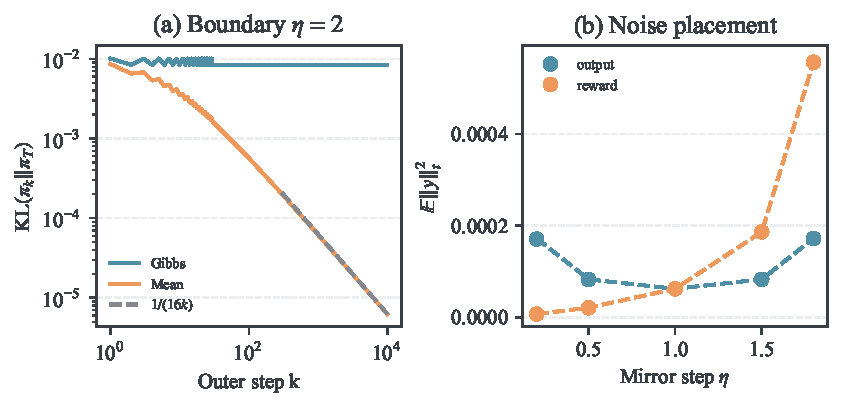
\includegraphics[width=0.96\textwidth]{../../results/hard-sync-audit/hard-sync.pdf}
 \caption{固定三元词表下的 hard-sync 审计。左：$\eta=2$ 的精确 Gibbs 与 Mean teacher KL；右：固定输出噪声和固定 reward 噪声的 teacher 加权二阶矩。点和实线来自数值更新，虚线来自独立理论预测。}
 \label{fig:hard-sync-audit}
\end{figure}

实验中的浮点求根和有限时间误差不替代证明。相反，精确恒等式、局部阶数、边界常数与随机二阶矩分别给出四类独立的数值约束，使实现错误能被具体定位。配置、源码版本、脚本校验和及最大残差记录在 \path{metadata.json}，完整复现命令与逐项结果见实验报告。

